\documentclass[journal,12pt,twocolumn]{IEEEtran}

\usepackage{enumitem}
\usepackage{amsmath}
\usepackage{amssymb}
\usepackage{gensymb}
\usepackage{graphicx}
\usepackage{txfonts}         
\usepackage{listings}
\usepackage{lstautogobble}
\usepackage{mathtools}
\usepackage{bm}
\usepackage{hyperref}
\usepackage{polynom}
\usepackage{siunitx}
\usepackage{verbatim}
\usepackage[siunitx]{circuitikz}

\newcommand{\solution}{\noindent \textbf{Solution: }}
\providecommand{\pr}[1]{\ensuremath{\Pr\left(#1\right)}}
\providecommand{\brak}[1]{\ensuremath{\left(#1\right)}}
\providecommand{\cbrak}[1]{\ensuremath{\left\{#1\right\}}}
\providecommand{\sbrak}[1]{\ensuremath{\left[#1\right]}}
\providecommand{\mean}[1]{E\left[ #1 \right]}
\providecommand{\var}[1]{\mathrm{Var}\left[ #1 \right]}
\providecommand{\der}[1]{\mathrm{d} #1}
\providecommand{\gauss}[2]{\mathcal{N}\ensuremath{\left(#1,#2\right)}}
\providecommand{\mbf}{\mathbf}
\providecommand{\abs}[1]{\left\vert#1\right\vert}
\providecommand{\norm}[1]{\left\lVert#1\right\rVert}
\providecommand{\z}[1]{{\mathcal{Z}}\cbrak{#1}}
\providecommand{\ztrans}{\overset{\mathcal{Z}}{ \rightleftharpoons}}
\providecommand{\system}[1]{\overset{\mathcal{#1}}{ \longleftrightarrow}}
\providecommand{\parder}[2]{\frac{\partial}{\partial #2} \brak{#1}}

\let\StandardTheFigure\thefigure
\let\vec\mathbf

\numberwithin{equation}{section}
\numberwithin{figure}{section}
%\renewcommand{\thefigure}{\theenumi}
\renewcommand\thesection{\arabic{section}}

\newcommand{\myvec}[1]{\ensuremath{\begin{pmatrix}#1\end{pmatrix}}}
\newcommand{\mymat}[1]{\ensuremath{\begin{bmatrix}#1\end{bmatrix}}}
\newcommand{\mydet}[1]{\ensuremath{\begin{vmatrix}#1\end{vmatrix}}}
\newcommand{\define}{\stackrel{\triangle}{=}}

\DeclareMathOperator*{\argmin}{arg\,min}
\DeclareMathOperator*{\argmax}{arg\,max}

\makeatletter
\def\pld@CF@loop#1+{%
    \ifx\relax#1\else
        \begingroup
          \pld@AccuSetX11%
          \def\pld@frac{{}{}}\let\pld@symbols\@empty\let\pld@vars\@empty
          \pld@false
          #1%
          \let\pld@temp\@empty
          \pld@AccuIfOne{}{\pld@AccuGet\pld@temp
                            \edef\pld@temp{\noexpand\pld@R\pld@temp}}%
           \pld@if \pld@Extend\pld@temp{\expandafter\pld@F\pld@frac}\fi
           \expandafter\pld@CF@loop@\pld@symbols\relax\@empty
           \expandafter\pld@CF@loop@\pld@vars\relax\@empty
           \ifx\@empty\pld@temp
               \def\pld@temp{\pld@R11}%
           \fi
          \global\let\@gtempa\pld@temp
        \endgroup
        \ifx\@empty\@gtempa\else
            \pld@ExtendPoly\pld@tempoly\@gtempa
        \fi
        \expandafter\pld@CF@loop
    \fi}
\def\pld@CMAddToTempoly{%
    \pld@AccuGet\pld@temp\edef\pld@temp{\noexpand\pld@R\pld@temp}%
    \pld@CondenseMonomials\pld@false\pld@symbols
    \ifx\pld@symbols\@empty \else
        \pld@ExtendPoly\pld@temp\pld@symbols
    \fi
    \ifx\pld@temp\@empty \else
        \pld@if
            \expandafter\pld@IfSum\expandafter{\pld@temp}%
                {\expandafter\def\expandafter\pld@temp\expandafter
                    {\expandafter\pld@F\expandafter{\pld@temp}{}}}%
                {}%
        \fi
        \pld@ExtendPoly\pld@tempoly\pld@temp
        \pld@Extend\pld@tempoly{\pld@monom}%
    \fi}
\makeatother

\lstset {
	frame=single, 
	breaklines=true,
	columns=fullflexible,
	autogobble=true
}             
                               
\title{Mobile Charger Lab Report \\ \Large EE3900: Linear Systems and Signal Processing \\ \large Indian Institute of Technology Hyderabad}
\author{Aakash Kamuju \\ \normalsize AI21BTECH11001 \\ \vspace*{20pt} }

\begin{document}

	\maketitle

	\section{Aim}
	The aim is to build a working mobile charger. The circuit must output \SI{5}{\volt} DC to charge a mobile phone after taking \SI{230}{\volt} AC as input.
	
	\section{Materials Required}
	\begin{itemize}
	\item 12-0-12 Tranformer
	\item 4 diodes
	\item \SI{100}{\micro\farad} Capacitor
	\item 7805 Regulator
	\item Output pin
	\item USB cable
	\end{itemize}

	\section{Circuit Diagram}
	\begin{figure}[!ht]
		\centering
		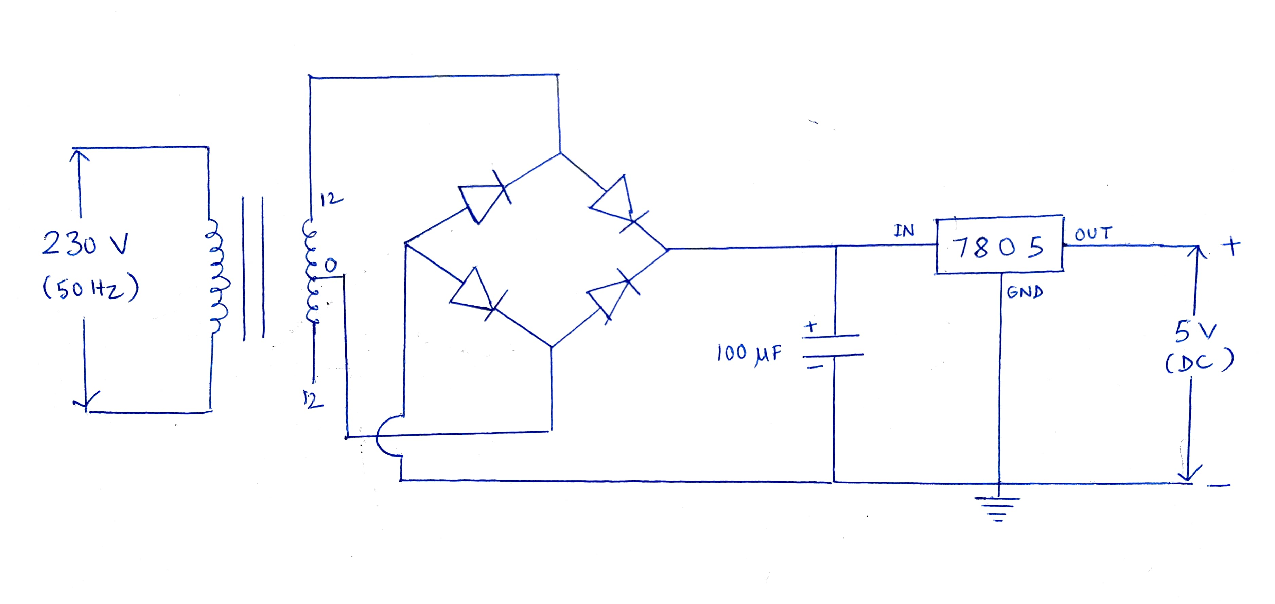
\includegraphics[width=\columnwidth]{./figs/circuit.pdf}
		\caption{Circuit diagram of a mobile charger}
		\label{fig-ckt}	
	\end{figure}
	
	\section{Circuit Explanation}
	\begin{itemize}
	\item The transformer steps down the \SI{230}{\volt} AC main supply to \SI{12}{\volt} AC. Note that these are RMS voltages. The peak voltage will thus be $12\sqrt{2} \approx \SI{20}{\volt}$. The transformed voltage is given by
	\begin{align}
		v(t) = \SI[parse-numbers=false]{12\sqrt{2}\sin(100\pi t + \phi)}{\volt}
	\end{align}
	\begin{figure}[!ht]
		\centering
		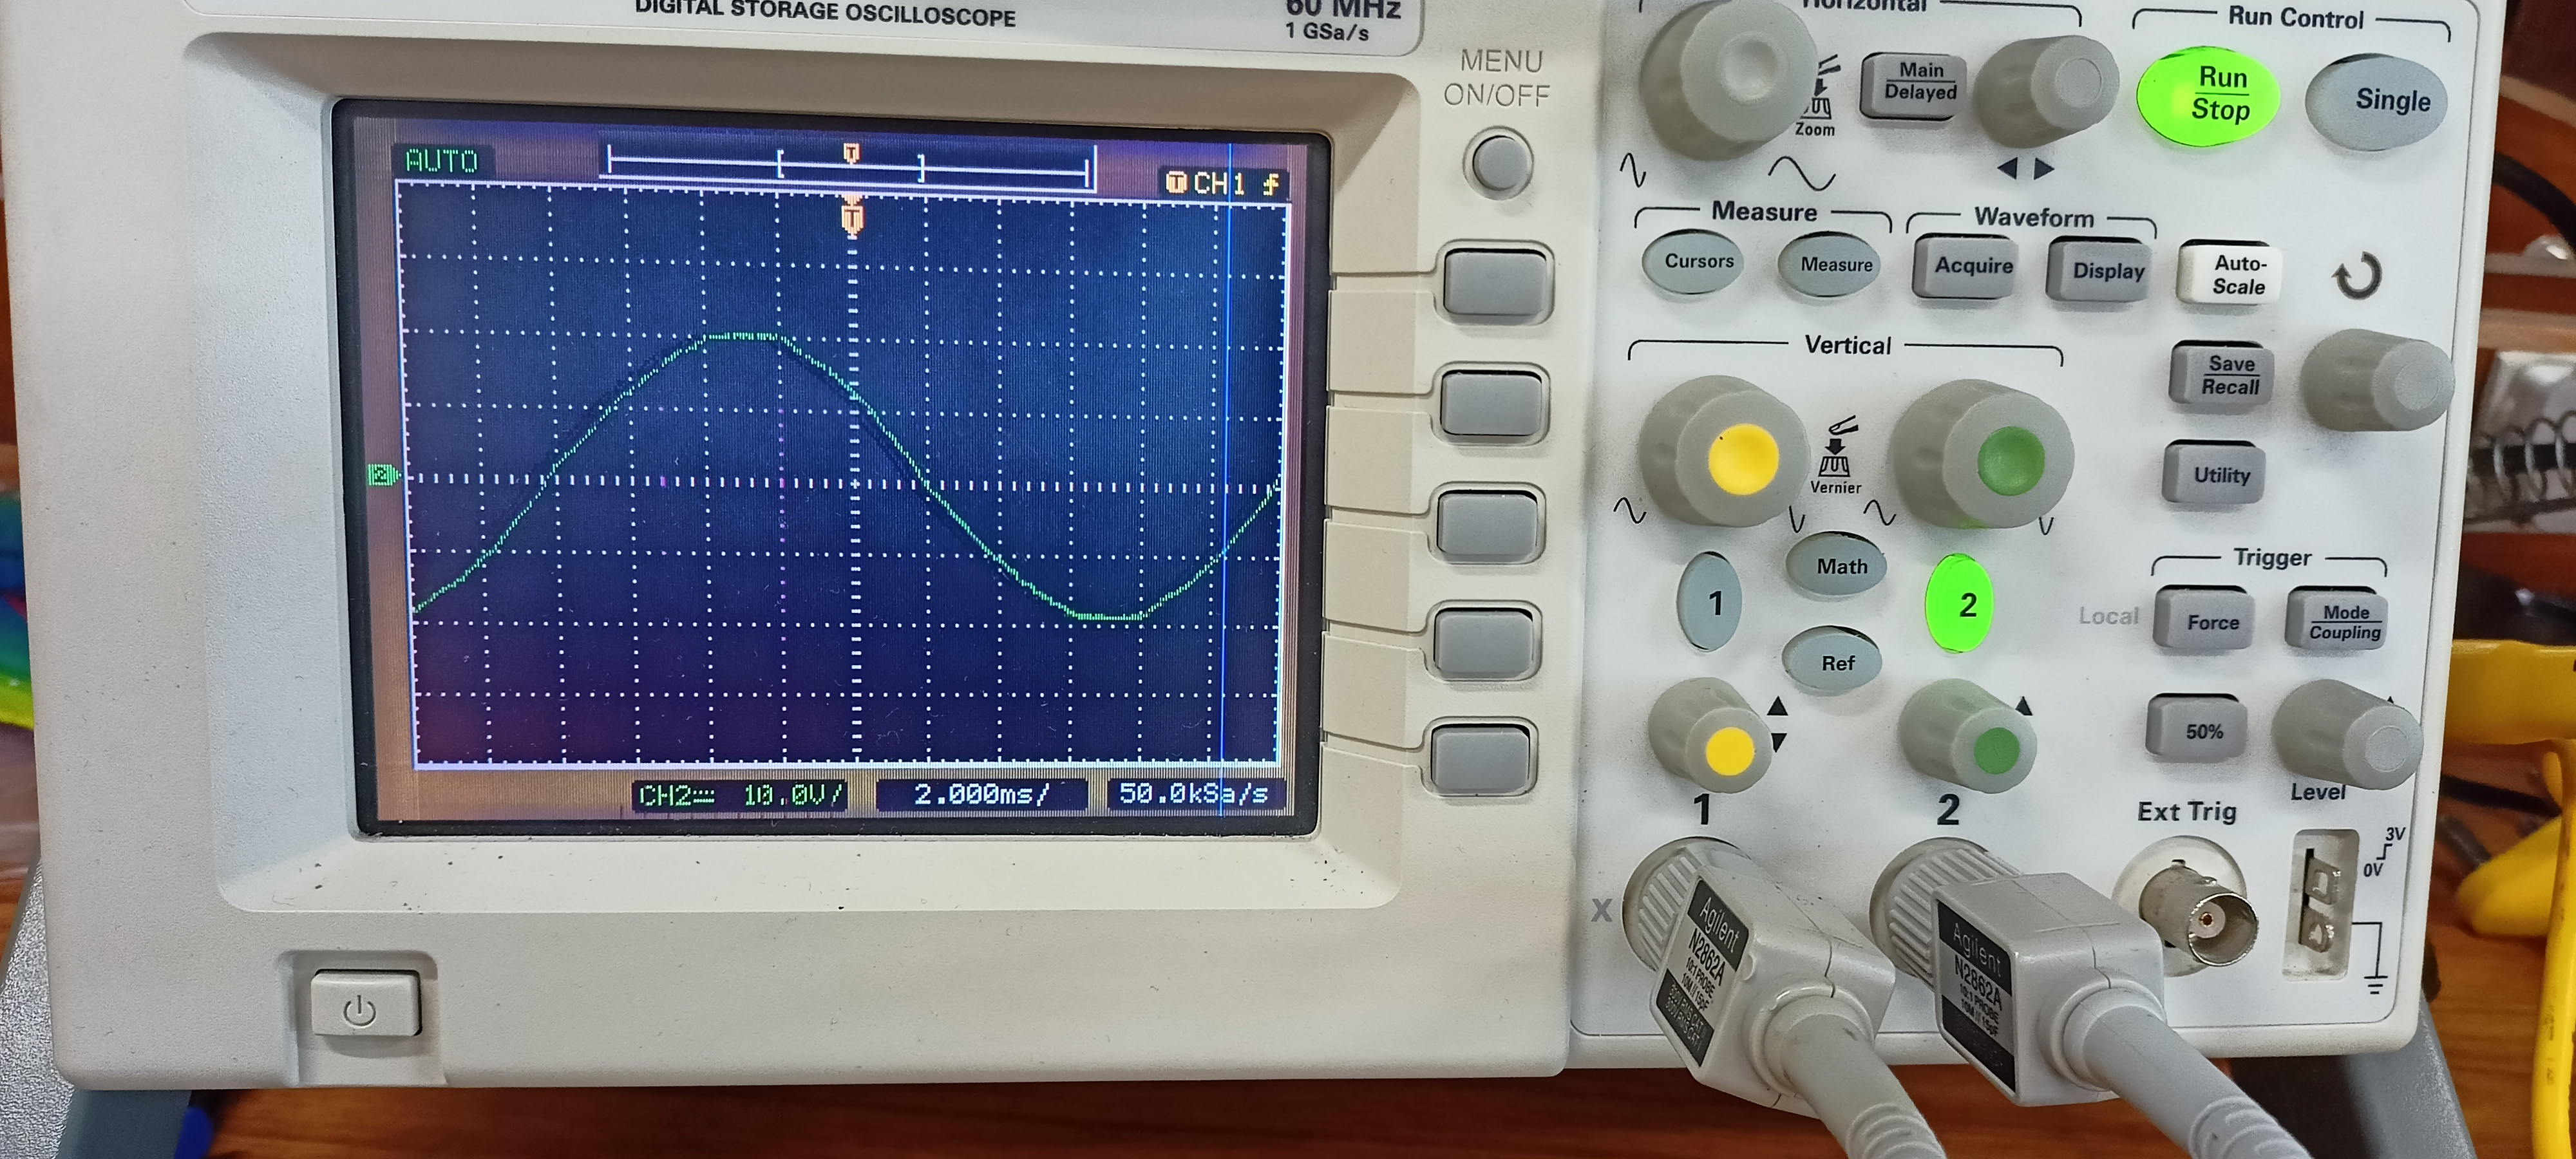
\includegraphics[width=\columnwidth]{./figs/transformer.jpg}
		\caption{CRO output after transformer}
		\label{fig-transformer}	
	\end{figure}
	
	\item The alternating current now passes through a bridge rectifier. The output is a pulsating DC wave whose peak is \SI[parse-numbers=false]{12\sqrt{2}}{\volt}. The voltage at this stage is given by
	\begin{align}
		v(t) = \SI[parse-numbers=false]{12\sqrt{2}\abs{\sin(100\pi t + \phi)}}{\volt}
	\end{align}

	\begin{figure}[!ht]
		\centering
		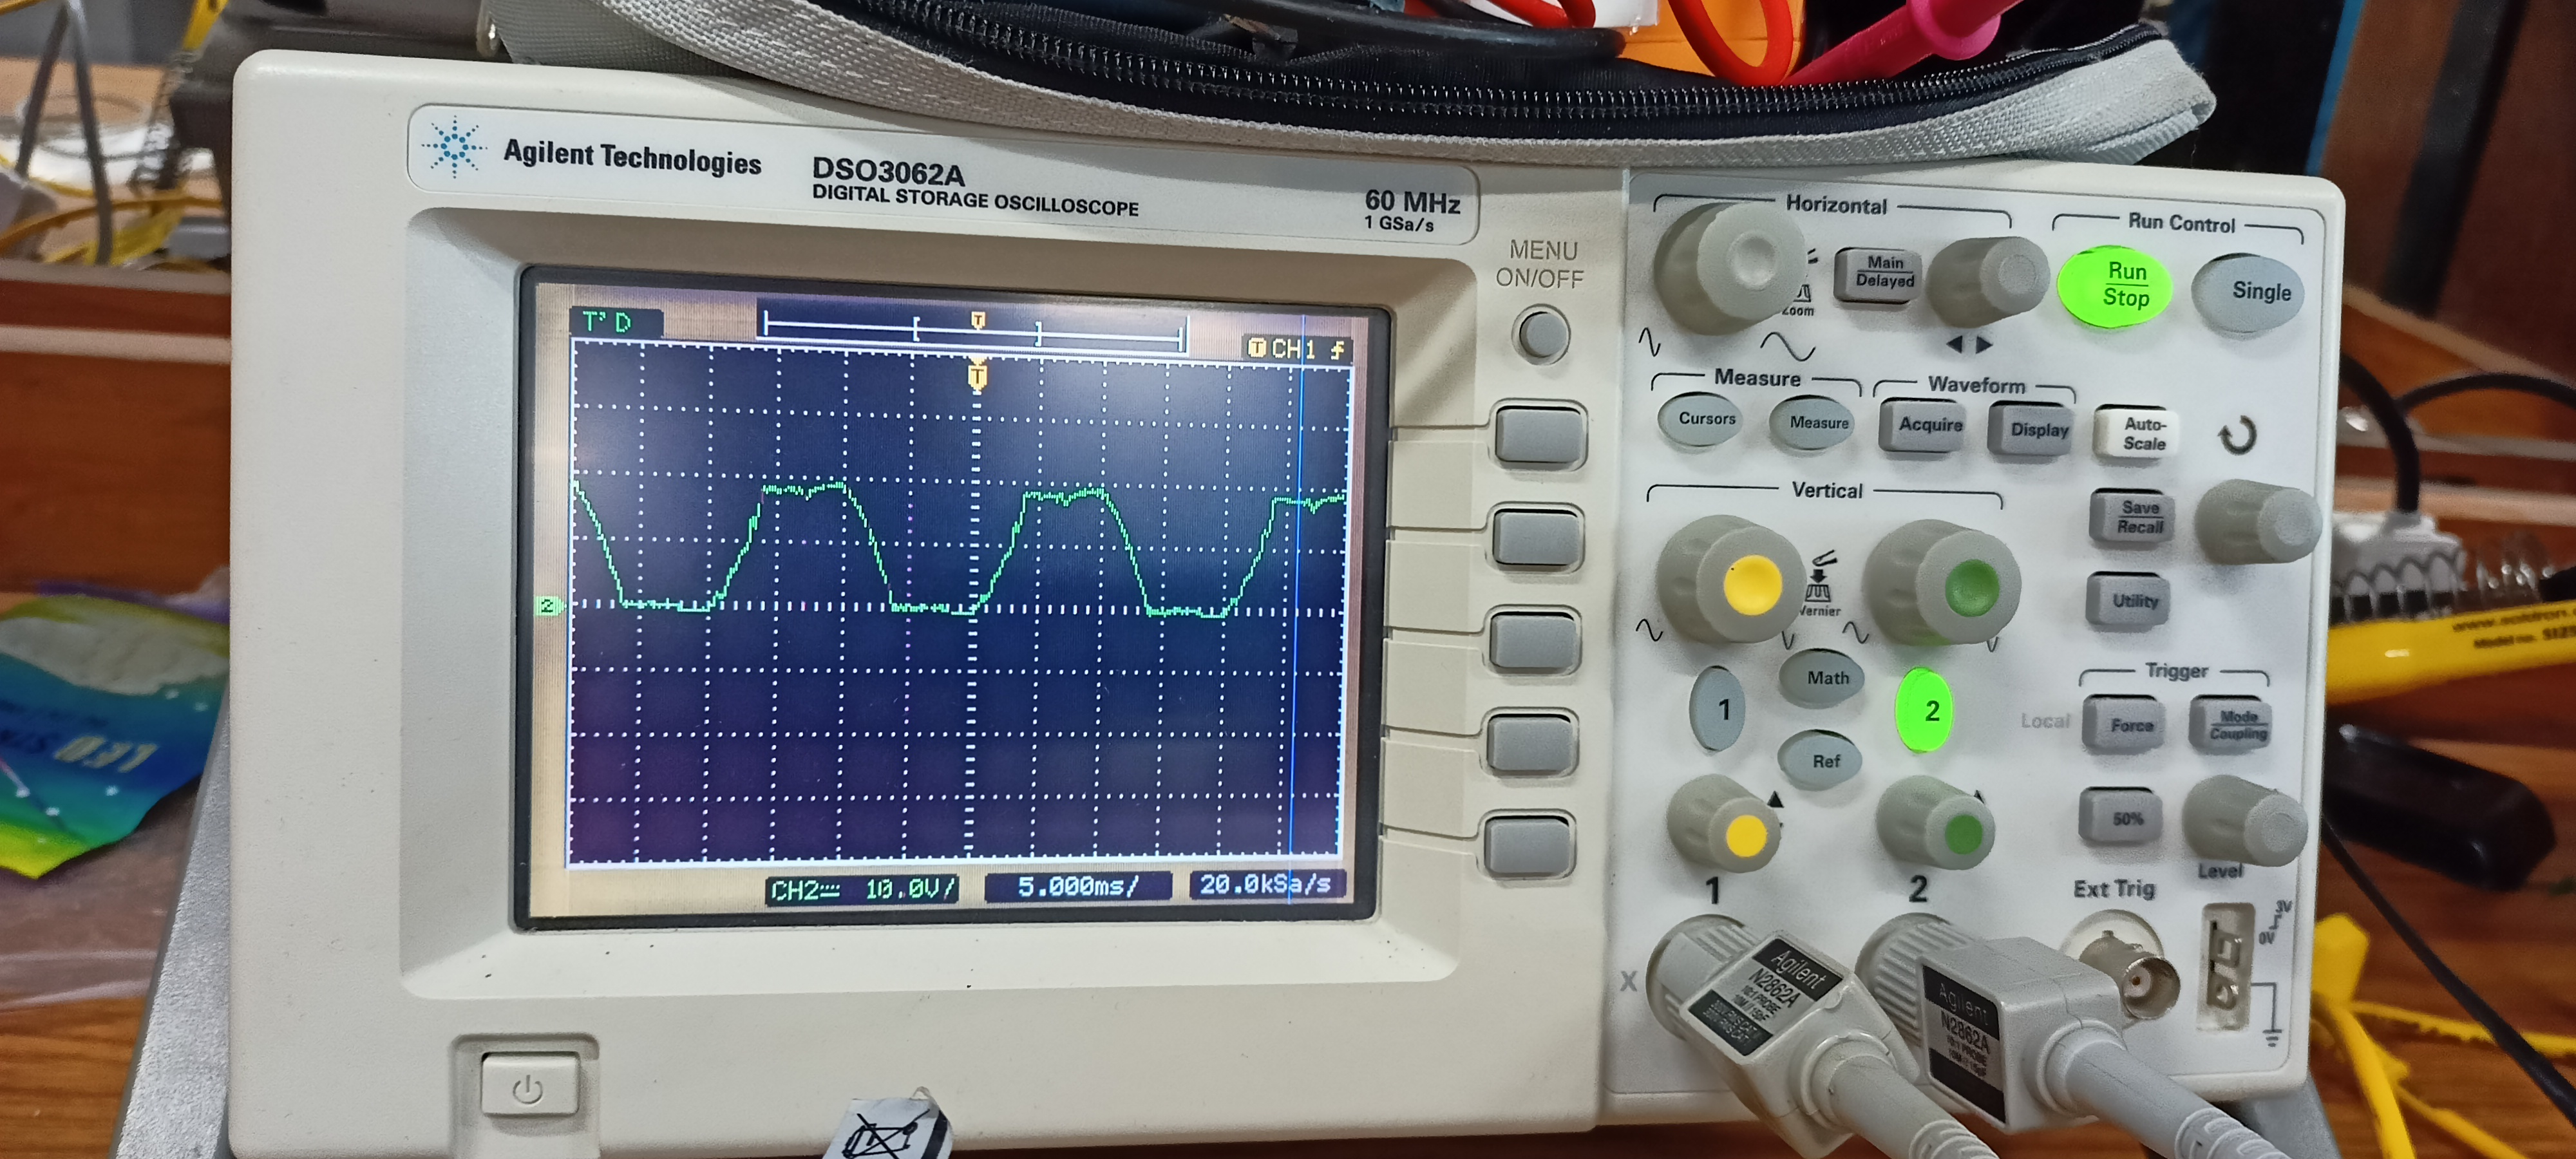
\includegraphics[width=\columnwidth]{./figs/rectifier-1.jpg}
		\caption{Rectified output}
		\label{fig-rectifier-1}	
	\end{figure}
	
	\item A capacitor is used as a low-pass filter here to choose only the zero frequency component thereby converting the current into pure DC of \SI[parse-numbers=false]{12\sqrt{2}}{\volt}
	\begin{align}
		v(t) = \SI[parse-numbers=false]{12\sqrt{2}}{\volt}
	\end{align}

	\begin{figure}[!ht]
		\centering
		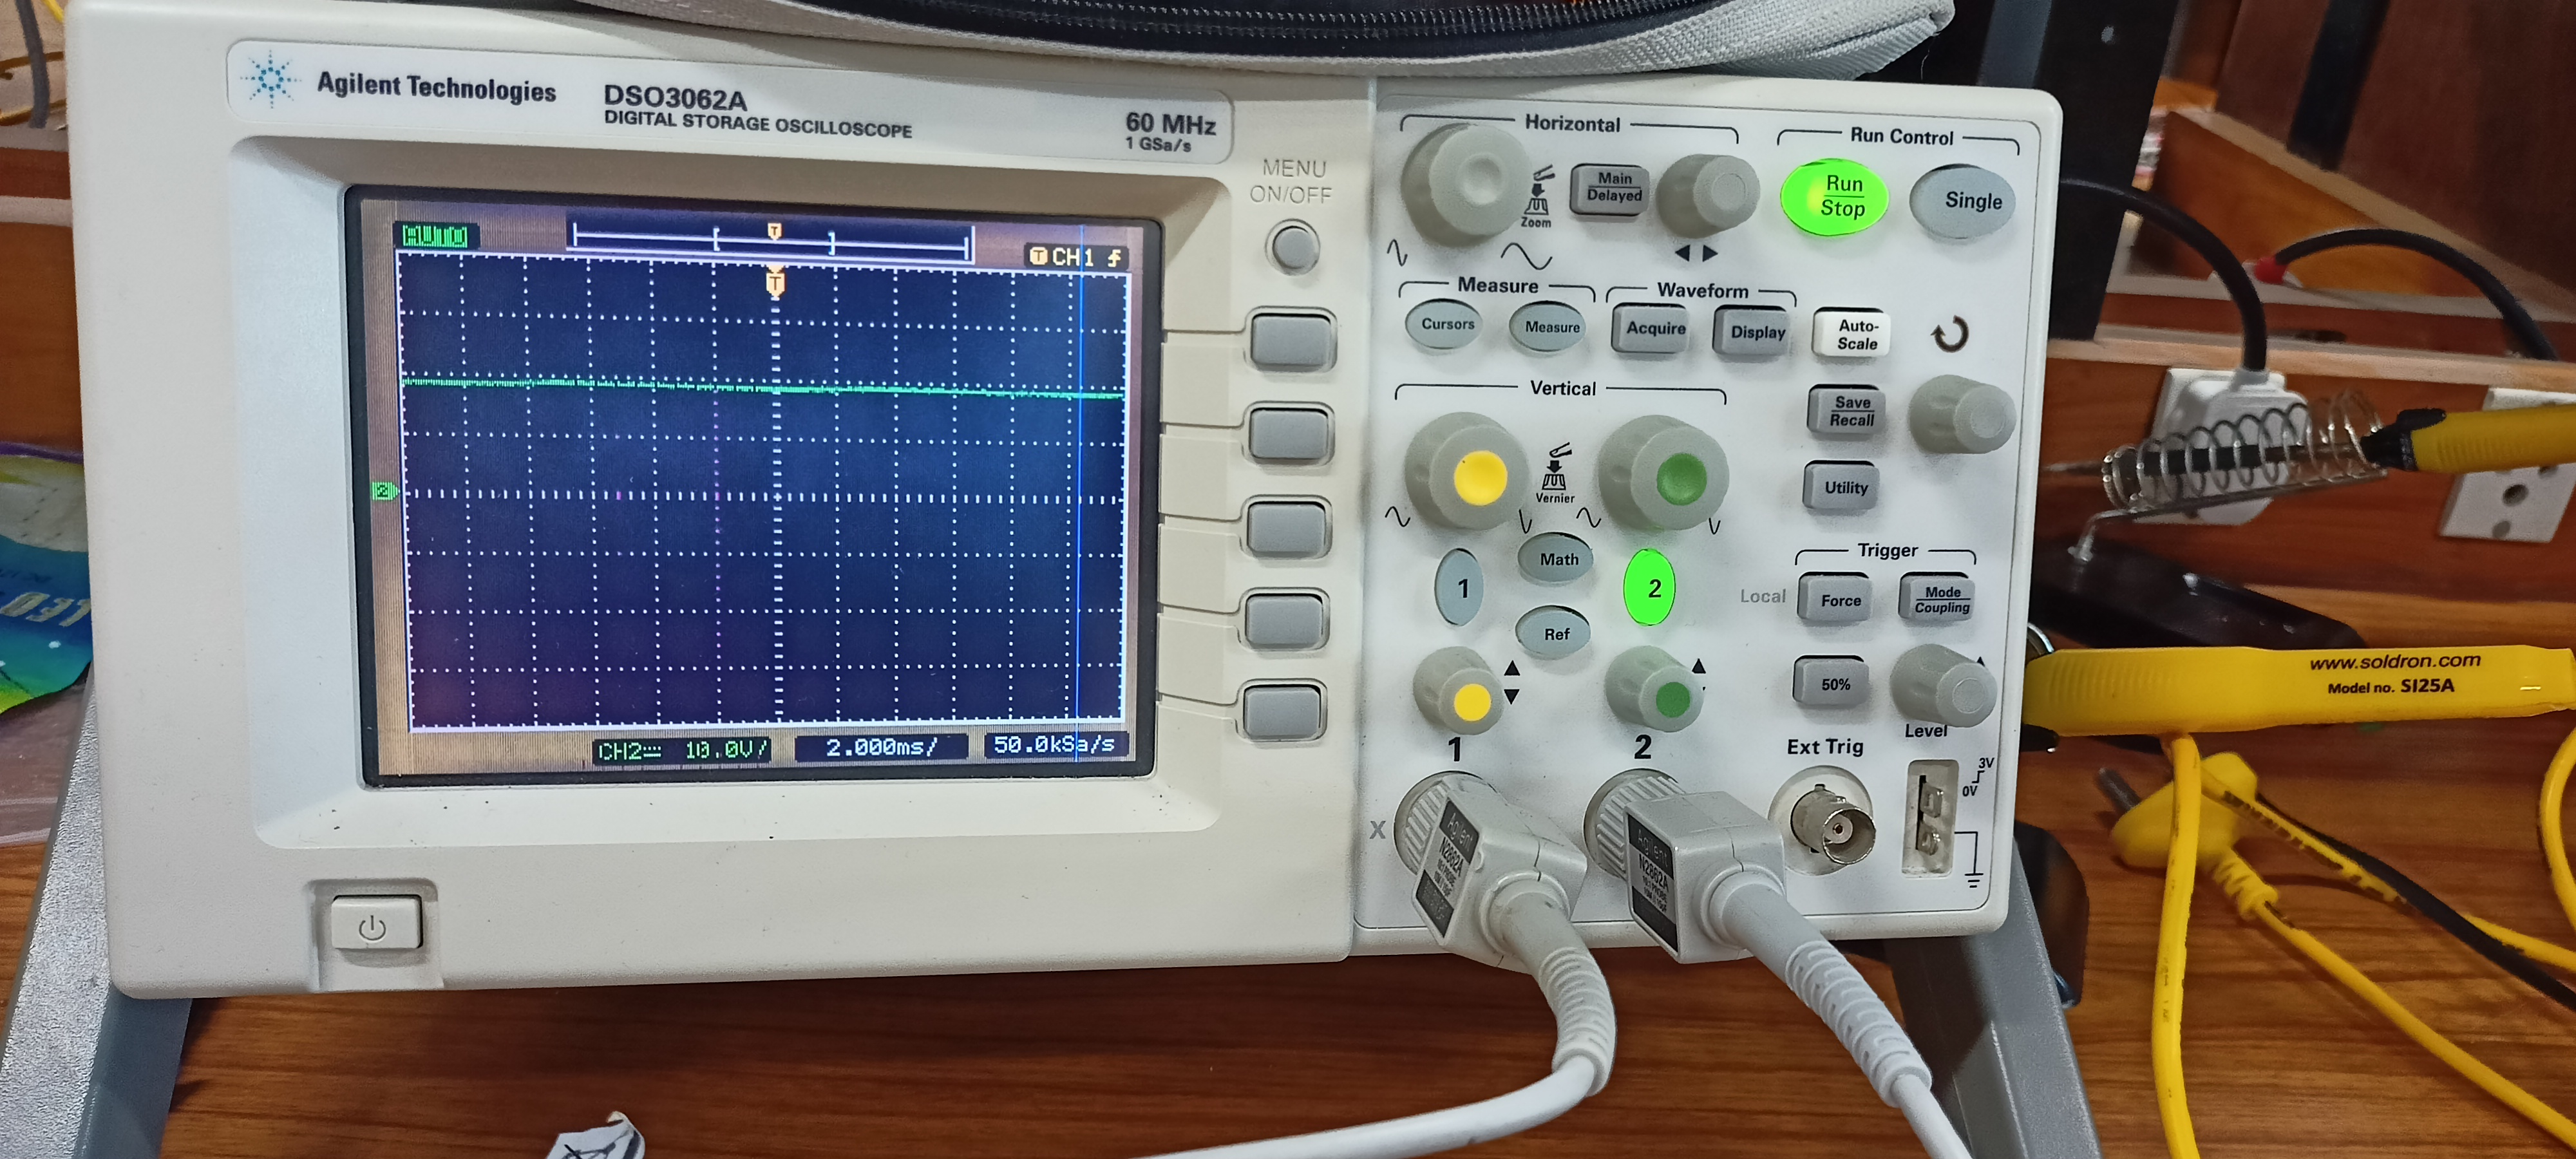
\includegraphics[width=\columnwidth]{./figs/filter.jpg}
		\caption{Filtered output}
		\label{fig-filter}	
	\end{figure}
	
	\item Finally, the 7805 regulator stabilizes the output by eliminating noise and converts it into \SI{5}{\volt} DC which is then used to charge the mobile phone.
	\begin{align}
		v(t) = \SI{5}{\volt}
	\end{align}
	\begin{figure}[!ht]
		\centering
		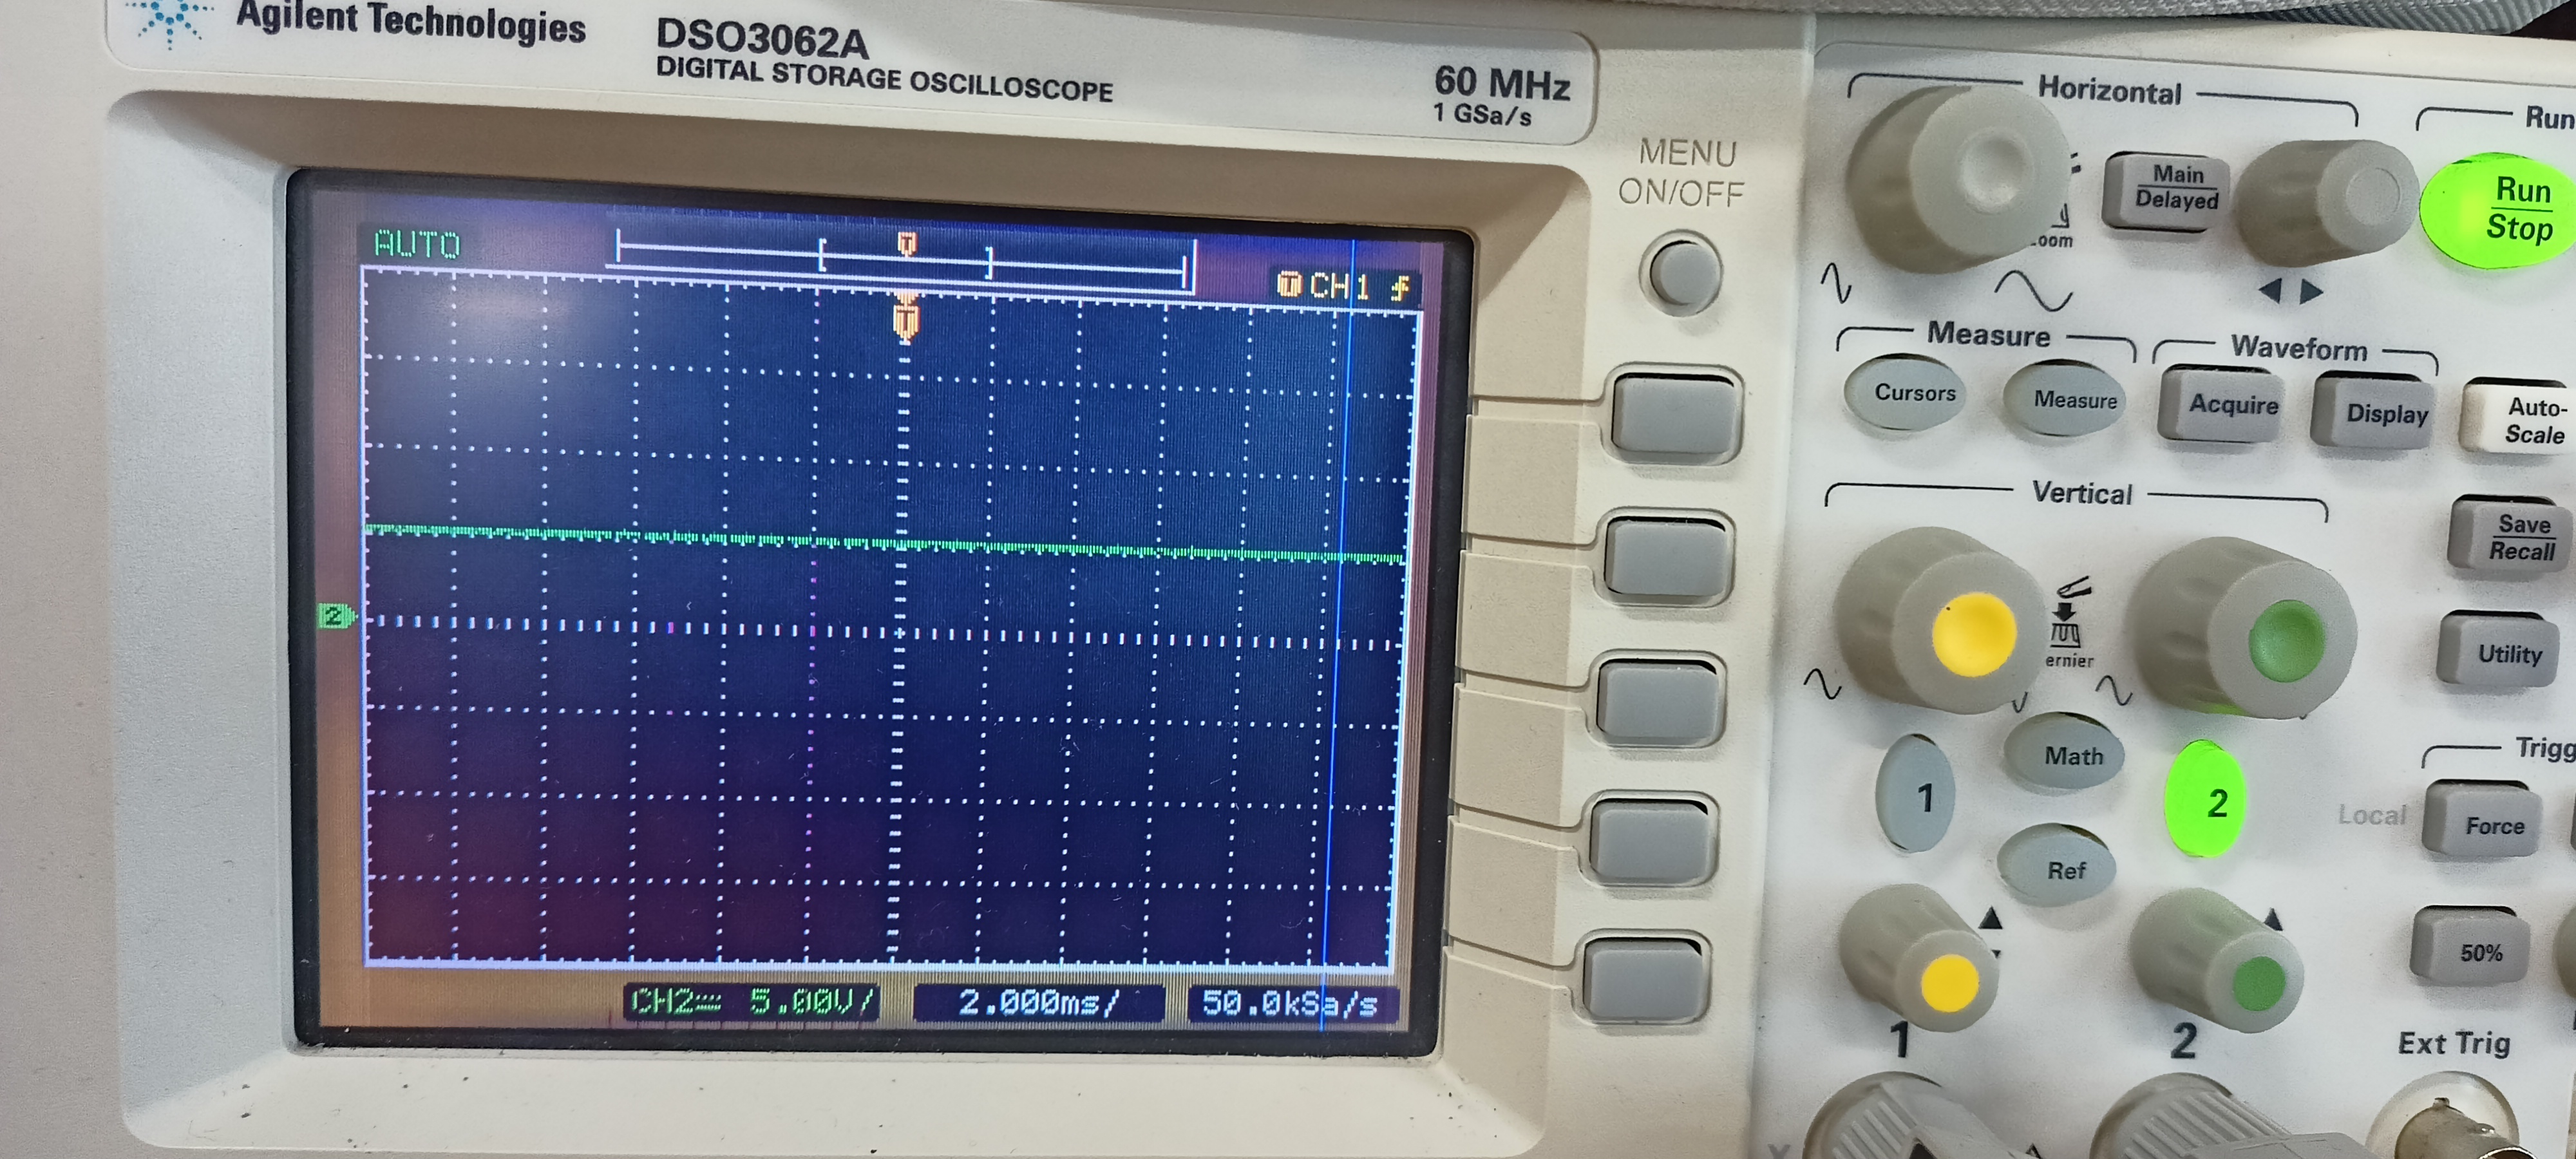
\includegraphics[width=\columnwidth]{./figs/regulator.jpg}
		\caption{Regulated output}
		\label{fig-regulator}	
	\end{figure}
	\end{itemize}
	
	\section{Observations}
	Using a multimeter, we can verify that the output obtained is indeed \SI{5}{\volt} DC.
	
	
	
	\end{document}
